%%=============================================================================
%% Inleiding
%%=============================================================================

\chapter{JavaScript frameworks vergelijking}
\label{ch:onderzoek}

In dit hoofdstuk zal mijn onderzoek uitgebreid uigelegd worden. Alle criteria die hiervoor besproken zijn zullen hier vergeleken worden met elkaar. Hieruit zal later een conclusie genomen worden. In de praktische vergelijking zullen ook de test applicaties grondig verduidelijkt worden.

\section{Theoretische vergelijking}
\label{sec:theoretische_vergelijking}

In dit onderdeel zal de theoretische vergelijking gemaakt worden aan de hand van de literatuurstudie. We gaan alle vergelijking criteria die besproken zijn in Hoofdstuk \ref{sec:Theoretische_Vergelijking} hier behandelen.

Alle resultaten zijn aanwezig in tabel \ref{table:theoretische_vergelijking}. Hieruit kunnen we de volgende conclusies halen.

\begin{itemize}
	\item React en Vue zijn het populairst op GitHub. Dit betekend dat er waarschijnlijk voor React en Vue meer online resources te vinden zijn. We kunnen hier ook uit afleiden dat er meer libraries ondersteund zullen worden door React en Vue.
	\item Angular heeft meer zoekresultaten op Google trends en stackoverflow trends. Dit betekend dat er meer vragen over Angular gesteld maar ook beantwoord kunnen worden.
	\item Security zit ingebouwd in Angular. Bij React en Vue zal de developer zelf nog maatregelen moeten treffen om security op punt te stellen.
	\item Angular en React worden gebruikt door grote bedrijven. Hierdoor tonen zei dat ze vertrouwen hebben in dit framework en zal er een groter publiek naar deze frameworks getrokken worden.
	\item Angular legt een bepaald ontwerppatroon op bij de developer. React en Vue doen dit niet waardoor ze meer vrijheid creëren. In Angular kunnen er veel fouten voorkomen worden net door dit ontwerppatroon.
	\item Op alle andere vlakken scoren de drie frameworks gelijk.
\end{itemize}

\begin{table}[]
	\centering
	\caption{Theoretische vergelijking}
	\label{table:theoretische_vergelijking}
	\begin{tabular}{|p{7cm}||p{2cm}|p{2cm}|p{2cm}|}
		\hline
		&Angular &Vue   &React \\ \hline \hline
		Wat zijn de resultaten op Google Trends van deze drie frameworks?
		&\multicolumn{3}{c|}{Figuur \ref{fig:google_trends}}\\ \hline
		Wat zijn de resultaten op StackOverflow Trends van deze drie frameworks?
		&\multicolumn{3}{c|}{Figuur \ref{fig:stackoverflow_trends}}\\ \hline
		Hoeveel GitHub watchers telt het framework? \autocite{github_front-end_????} 
		&3040     &4927  &5850 \\ \hline
		Voorkomt het framework Cross Site Request Forgery? \autocite{_angular_2018-1}
		&Ja         &Nee    &Nee \\ \hline
		Voorkomt het framework Cross Site Scripting? \autocite{_angular_2018-1}
		&Ja         &Nee    &Nee \\ \hline
		Bestaat er een tool om code te genereren?
		&Ja         &Ja     &Ja       \\ \hline
		Wordt het framework gebruikt door een grote organisatie? \autocite{_made_????} \autocite{_made_????-1}
		&Ja         &Geen kwaliteitsvolle bronnen &Ja \\ \hline
		Ondersteunt het framework mobiele apparaten?
		&Ja         &Ja     &Ja       \\ \hline
		Heeft de framework een specifiek ontwerp patroon waardoor het development van verschillende lagen of componenten makkelijker word?
		&Ja         &Nee   &Nee       \\ \hline
		Ondersteund het framework een component gebaseerde methodologie?
		&Ja         &Ja     &Ja       \\ \hline
		Ondersteund het framework unit tests? \autocite{_testing_2018} \autocite{_testing_2018-2} \autocite{_testing_2018-1}
		&Ja         &Ja     &Ja       \\ \hline
		Ondersteund het framework integratie tests?
		&Ja         &Ja     &Ja      \\  \hline
	\end{tabular}
\end{table}

\begin{figure}[h]
	\caption{Angular, Vue en React google trends relatie}
	\centering
	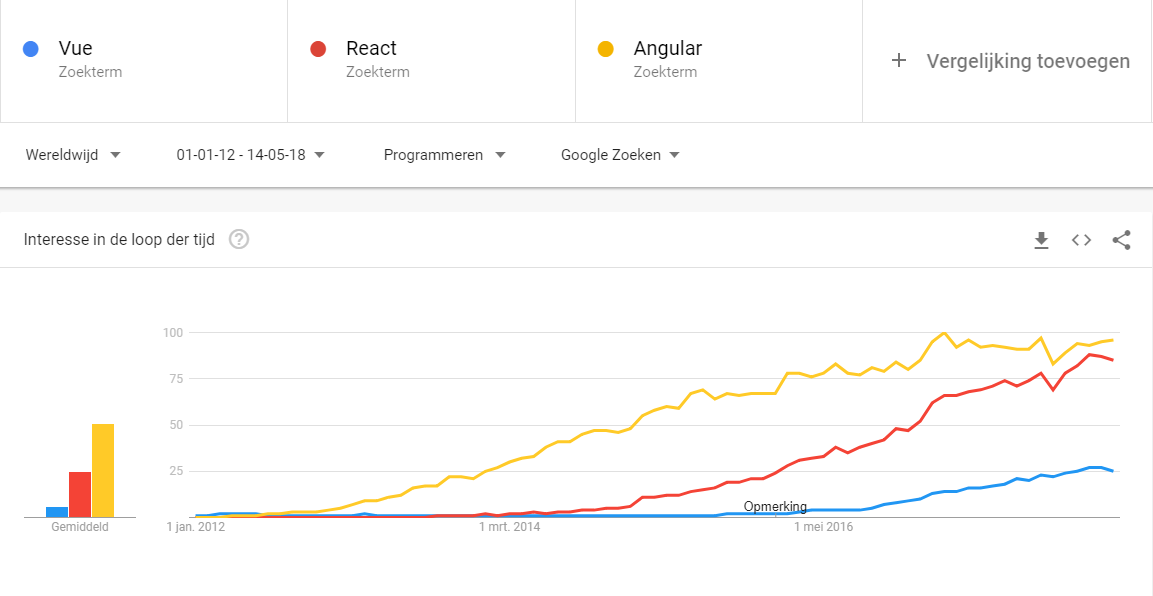
\includegraphics[width=1\textwidth]{img/googleTrends.png}
	\label{fig:google_trends}
\end{figure}

\begin{figure}[h]
	\caption{Angular, Vue en React stackoverflow trends relatie}
	\centering
	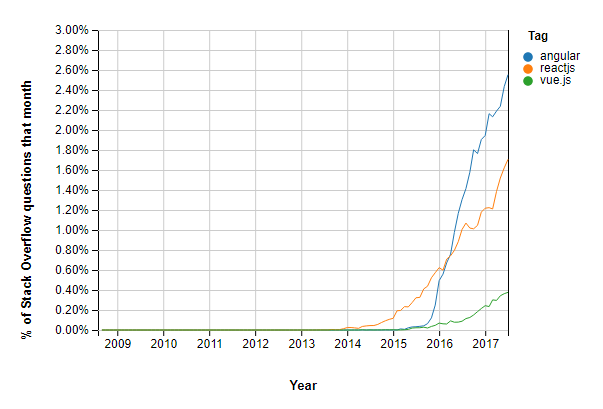
\includegraphics[width=0.6\textwidth]{stackoverflowTrends.png}
	\label{fig:stackoverflow_trends}
\end{figure}


\section{Praktische vergelijking}
\label{sec:praktische_vergelijking}
In dit onderdeel worden alle praktische vergelijkingen gemaakt. Dit word gedaan door de resultaten van de performance tests en software complexiteit te vergelijken.

Om alle tests zo eerlijk en correct mogelijk te laten verlopen zullen we onze omgevingsfactoren gelijk stellen bij alle tests. De tests die uitgevoerd worden in dit onderzoek zijn uitgevoerd met volgende setup:

\begin{itemize}
	\item Windows 10 Home 64 bits (10.0, build16299)
	\item Intel Core i7-4790 CPU @ 3.6GHz
	\item 8GB RAM
	\item Google Chrome 66.0.3359.139
\end{itemize}

Bij elke test zullen alle mogelijke processen op de pc gestopt worden behalve de browser.

\subsection{Grootte}
\label{sec:grootte}

Hier zullen de filesizes besproken worden die in de netwerk tab van de browser gedownload moeten worden. De software die hiervoor gebruikt werd is Google Chrome developer tools netwerk tab. Er werd hier geen gebruik gemaakt van een shortlist omdat deze keuze de meest logische is. Andere software zal ook hetzelfde resultaat geven. Er zijn ook geen voor of nadelen aan.

In tabel \ref{table:file_sizes} zien we dat React en Vue zeer sterk bij elkaar liggen met amper 30 kilobytes verschil. Angular daarentegen heeft een geweldige grootte van 3160 kilobytes. De reden hiervoor is omdat Angular een compleet framework meestuurd. Als deze applicaties groter zouden zijn dan zou het verschil kleiner geweest zijn. Dit is iets waar in het begin van deze tests geen rekening mee gehouden is maar waar wel veel uit geleerd kan worden.

\begin{table}[]
	\centering
	\caption{Grootte in kilobytes}
	\label{table:file_sizes}
	\begin{tabular}{|c|c|c|} \hline
		Angular &Vue   &React \\ \hline
		3160     &90.3  &128.4 \\ \hline
	\end{tabular}
\end{table}

\subsection{First meaningfull paint}
\label{sec:first_meaningfull_paint}

In dit onderdeel zullen we de first meaningfull paint resultaten bespreken. Elke test is tien keer uitgevoerd op elke pagina. De first meaningfull paint is de tijd waarop de pagina het eerst zichtbaar wordt. Deze test werd maar tien keer uitgevoerd omdat deze waarde nooit veel zal verschillen op elke computer in perfecte omstandigheden. De software die hiervoor gebruikt werd is lighthouse audits van Google Chrome developer tools. De reden waarom er niet geopteerd word voor een shortlist is omdat google lighthouse de enigen zijn die deze functionaliteit op het moment van schrijven bieden.

In tabel \ref{table:first_meaningfull_paint} zien we dat Vue en React weer zeer sterke competitie voeren met elkaar. Angular is hier ook weer de uitzondering met tijden die tien keer langer duren dan Vue en React. De reden hiervoor is omdat de software die gebruikt is om deze tijden te meten langer zal laden hoe groter de grootte van het bestand is. Dit is een gevolg uit de test in het vorige hoofdstuk \ref{sec:grootte}.

\begin{table}[]
	\centering
	\caption{First meaningfull paint in milliseconden}
	\label{table:first_meaningfull_paint}
	\begin{tabular}{|c|c|c|c|} \hline
									&Angular       &Vue        &React      \\ \hline
		gemiddelde			&20270.00     &1845.00  &2304.00 \\ \hline
		minimuum			&19890.00     &1810.00  &2200.00  \\ \hline
		maximuum			&20870.00    &1890.00  &2500.00 \\ \hline
		mediaan				   &20230.00    &1840.00  &2295.00 \\ \hline
		standaarddeviatie &340.94        &24.187    &84.758    \\ \hline
	\end{tabular}
\end{table}

\subsection{Tarief}
\label{sec:tarief}







